\documentclass[border=3pt,tikz]{standalone}
\usepackage{amsmath}
\usetikzlibrary{calc}
\usetikzlibrary{arrows.meta} % for arrow size
\usetikzlibrary{calc}
\begin{document}
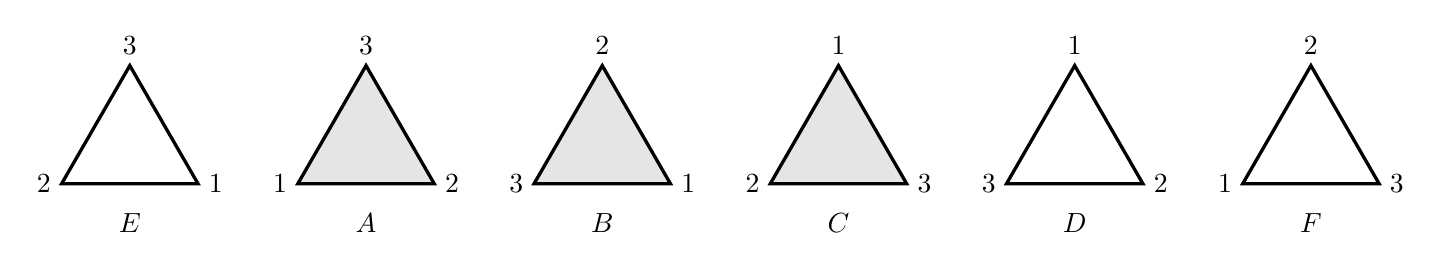
\begin{tikzpicture}[scale=1, extended line/.style={shorten >=-#1,shorten <=-#1},
    extended line/.default=1cm]
    \begin{scope}[]
        \coordinate (P3) at (0, 1);
        \coordinate (P2) at ({-sqrt(3)/2}, -0.5);
        \coordinate (P1) at ({sqrt(3)/2}, -0.5);
        
        \draw[very thick] (P1) node [right] {$1$}-- (P2) node[left] {$2$} -- (P3) node [above] {$3$} -- cycle;
    \end{scope}
        \node [] at (0, -1) {$E$};

    \begin{scope}[xshift=3cm]
    
        \coordinate (P1) at (0, 1);
        \coordinate (P2) at ({-sqrt(3)/2}, -0.5);
        \coordinate (P3) at ({sqrt(3)/2}, -0.5);
        \fill[fill=gray!20] (P1)--(P2)--(P3);
        \draw[very thick] (P1) node [above] {$3$}-- (P2) node[left] {$1$} -- (P3) node [right] {$2$} -- cycle;
        \node [] at (0, -1) {$A$};
    \end{scope}

    \begin{scope}[xshift=6cm]
    
        \coordinate (P1) at (0, 1);
        \coordinate (P2) at ({-sqrt(3)/2}, -0.5);
        \coordinate (P3) at ({sqrt(3)/2}, -0.5);
        \fill[fill=gray!20] (P1)--(P2)--(P3);
        \draw[very thick] (P1) node [above] {$2$}-- (P2) node[left] {$3$} -- (P3) node [right] {$1$} -- cycle;
        \node [] at (0, -1) {$B$};
    \end{scope}

    \begin{scope}[xshift=9cm]
    
        \coordinate (P1) at (0, 1);
        \coordinate (P3) at ({-sqrt(3)/2}, -0.5);
        \coordinate (P2) at ({sqrt(3)/2}, -0.5);
        \fill[fill=gray!20] (P1)--(P2)--(P3);
        \draw[very thick] (P1) node [above] {$1$}-- (P2) node[right] {$3$} -- (P3) node [left] {$2$} -- cycle;
        
        \node [] at (0, -1) {$C$};
    \end{scope}

    \begin{scope}[xshift=12cm]
    
        \coordinate (P1) at (0, 1);
        \coordinate (P3) at ({-sqrt(3)/2}, -0.5);
        \coordinate (P2) at ({sqrt(3)/2}, -0.5);
        
        \draw[very thick] (P1) node [above] {$1$}-- (P2) node[right] {$2$} -- (P3) node [left] {$3$} -- cycle;
        
        \node [] at (0, -1) {$D$};
    \end{scope}

    \begin{scope}[xshift=15cm]
    
        \coordinate (P2) at (0, 1);
        \coordinate (P1) at ({-sqrt(3)/2}, -0.5);
        \coordinate (P3) at ({sqrt(3)/2}, -0.5);
        
        \draw[very thick] (P1) node [left] {$1$}-- (P2) node[above] {$2$} -- (P3) node [right] {$3$} -- cycle;
        
        \node [] at (0, -1) {$F$};
    \end{scope}
    \end{tikzpicture}
\end{document}